\documentclass[addpoints,12pt]{exam}
%\documentclass[12pt]{article}
\usepackage[letterpaper, margin=0.75in]{geometry}
\usepackage{graphicx}
\usepackage{enumitem}
\usepackage{booktabs}
\usepackage{tabularx}
\usepackage{color}
\usepackage{wrapfig}

\begin{document}
\footer{}{Page \thepage\ of \numpages}{}


\begin{center}

\includegraphics[width=10cm]{../images/logo.png}
\end{center}

\begin{center}
\noindent{\LARGE Conceptual Physics \\ First Partial Test\\ \textbf{SOLUTIONS} \\ March 30, 2018 \\}
\end{center}


 
\clearpage

\begin{flushright}
Score: \hspace{0.2in} / \numpoints ~ points
\end{flushright}

\begin{questions}
\question \textbf{Binary Star Systems:} In solar systems like ours, there is one star (our sun) orbited by planets. However, other systems exist in which there are \textit{two} stars orbiting each other: These are known as \textit{binary star systems.} In binary star systems, both stars follow a (roughly) elliptical path. In the diagram below, images (I), (II), (III) and (IV) show snapshots in time of 2 stars in a binary system as they orbit each other. Use these images to answer the following questions. \textbf{For each question, please also \textit{explain your answer}.}

\begin{center}\input{../images/binary_star.pdf_tex}\end{center}

\begin{parts}
\part[2] At which instant (I, II, III, IV) is the \textit{gravitational force} between the two stars the \textit{greatest}? \textbf{Why?}
	\begin{TheSolution}
	\textbf{III.} The gravitational force is strongest when the two are closest together.
	\end{TheSolution}
\part[2] At which instant (I, II, III, IV) is the \textit{gravitational potential energy} between the two stars the \textit{greatest}? \textbf{Why?}
	\begin{TheSolution}
		\textbf{I.} Since gravity is an attractive force, the potential energy is strongest when the two are farthest apart.
	\end{TheSolution}
\part[2] Assume energy is conserved in a binary system. At which instant (if any) is the \textit{speed} of the two stars the \textit{greatest}? \textbf{Why?}
	\begin{TheSolution}
		\textbf{III.} The speed is greatest when the \textit{kinetic energy} is the greatest. The kinetic energy is the greatest when the potential energy is the smallest, which is when the two are closest together.
	\end{TheSolution}
\end{parts}

\clearpage

\question \textbf{Rutherford Experiment:} Also called the Geiger-Marsden experiment, was a landmark experiment that proved atoms contained a nucleus where the positive charge (and most of the mass) is concentrated. This was accomplished by bombarding very thin gold foils with ``alpha particles" (2 protons and 2 neutrons stuck together) and observing how the particles were deflected. The figure below shows an incoming alpha particle (positive charge) approaching a gold nucleus (also positively charged) and being deflected by their mutual repulsion. The gold nucleus remains nearly stationary during the event. Different parts of the particle's trajectory are labelled, and please use them to answer the following questions. \textbf{For each question, please also \textit{explain your answer}.}
	
	\noindent\begin{center}\input{../images/rutherford.pdf_tex}\end{center}
	
	\begin{parts}
	\part[2] At what point(s) during its trajectory (I, II, III, IV, V) does the alpha particle feel an electrical force, due to its interaction with the gold nucleus? \textbf{Why?}
		\begin{TheSolution}
			\textbf{All points.} The electric force has infinite range: at all points in space the two interact with each other (although as things get really far away, the force becomes vanishingly weak but \textit{never exactly zero})
		\end{TheSolution}
	\part[2] At what point(s) during its trajectory (I, II, III, IV, V) does the alpha particle experience the \textit{greatest electric force}? \textbf{Why?}
		\begin{TheSolution}
			\textbf{III.} The force is strongest when the two are closest together.
		\end{TheSolution}
	\part[2] At what point(s) during its trajectory (if any) does the alpha particle have the \textit{greatest electric potential energy}?\textbf{ Why?}
		\begin{TheSolution}
			\textbf{III.} Since the two particles are \textit{repelling} each other, the potential energy is greatest when the two are closest together.
		\end{TheSolution}
	\end{parts}

\clearpage
\question \textbf{Nuclear Fission:} Uranium is a radioactive element used as an energy source in nuclear reactors. When a uranium nucleus is bombarded with a neutron, it splits apart forming 2 other atoms, and in the process releases lots of nuclear potential energy (and more neutrons to continue the process).

\begin{center}
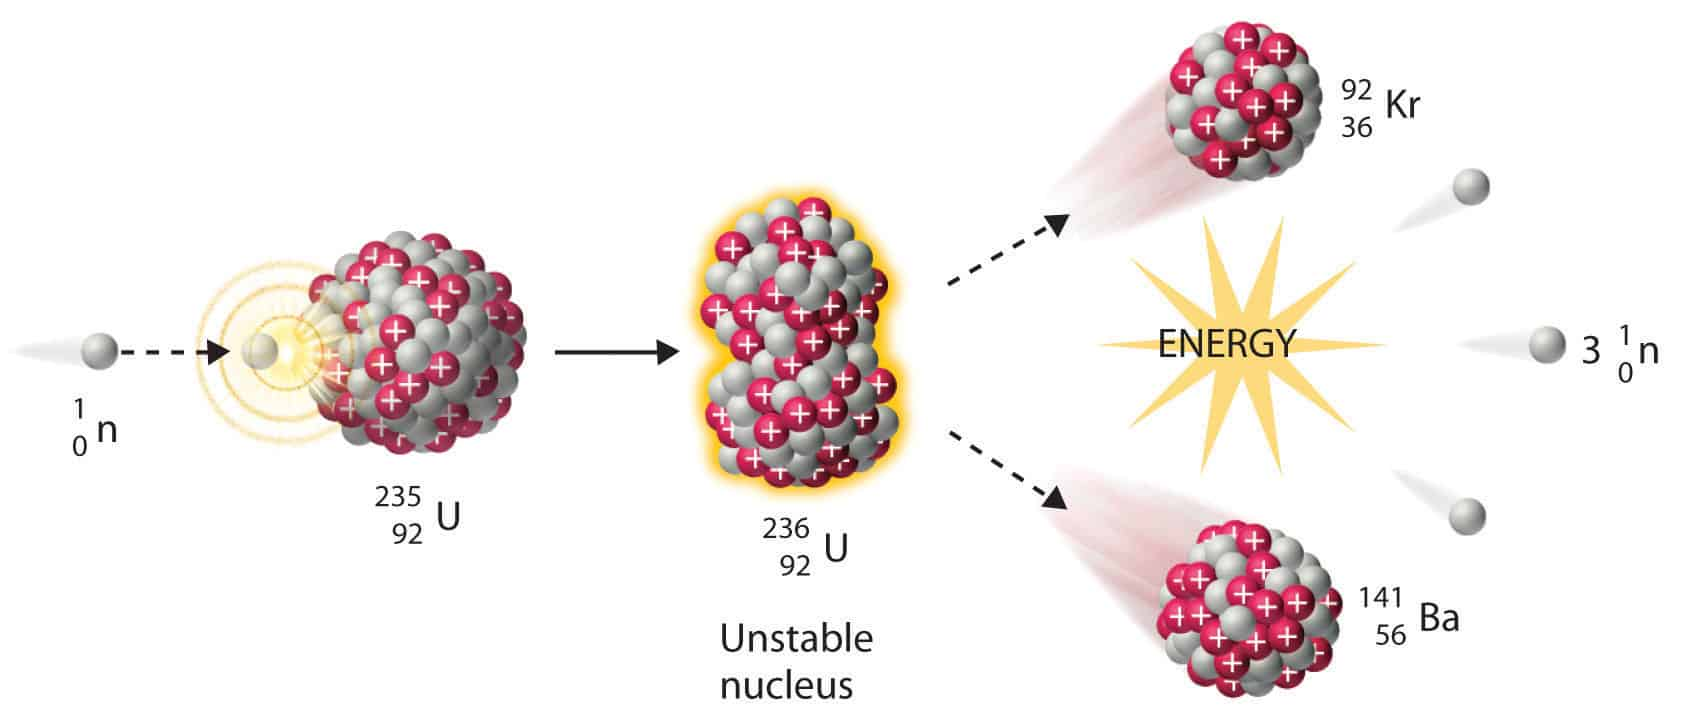
\includegraphics[width=0.8\textwidth]{../images/nuclear_fission.jpg}
\end{center}

\begin{parts}
	\part[2] The mass of 1 uranium atom is $4\times 10^{-22}$g. If a nuclear reactor has $8\times 10^{4}$g of uranium, how many atoms is this?
		\begin{TheSolution}
			\begin{eqnarray}
			\frac{8\times 10^{4}g}{4\times 10^{-22}g/atom} = 2\times 10^{26} atoms
			\end{eqnarray}
		\end{TheSolution}
	\part[2] The decay of 1 uranium atom releases $3\times 10^{-11}$J of energy. If all the atoms in the reactor were to decay, how much energy would be released?
		\begin{TheSolution}
			\begin{eqnarray}
				2\times 10^{26} atoms \times 3\times 10^{-11} J/atom = 6\times 10^{15} J
			\end{eqnarray}
		\end{TheSolution}
	\part[2] Burning the same amount of coal releases $2.4\times 10^{9}$J of energy. Which reaction produces more energy, burning coal or splitting uranium?
		\begin{TheSolution}
			\textbf{Splitting Uranium.} We look at the energy released by the two: $6\times 10^{15}$J vs. $2.4\times 10^{9}$J. The energy released by uranium is about 2.5 million times greater than coal.
		\end{TheSolution}
\end{parts}

\begin{minipage}{\linewidth}
\begin{wrapfigure}{R}{0.45\textwidth}
	\vspace{-20pt}
	\begin{center}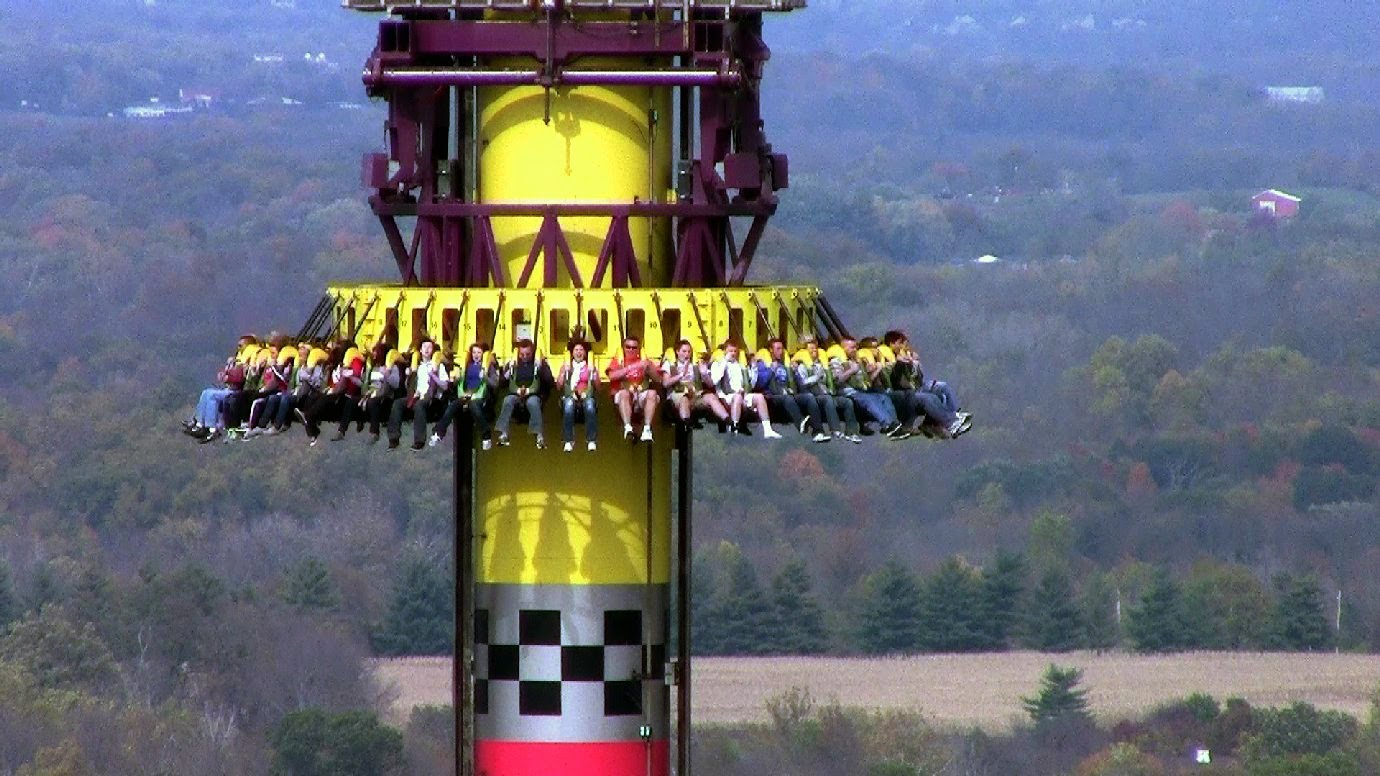
\includegraphics[width=0.4\textwidth]{../images/drop_tower_image.jpg}\end{center}
	\vspace{-20pt}
\end{wrapfigure}

\question \textbf{Drop Tower:} At theme parks, there is a kind of ride known as a \textit{drop tower.} People (safely strapped in harnesses) rise to the top of a large tower, and are then dropped down to experience free fall. The image to the right shows a picture of people on the drop-tower ride at Kings Island.

The graph below shows someone's \textit{velocity as a function of time} as they rise to the top (from 0 to 41 seconds), pause at the top not moving (from 41 to 52 seconds) and then falling (from 52 to 60 seconds). In all, the ride lasts exactly 1 minute.

\noindent\begin{center}
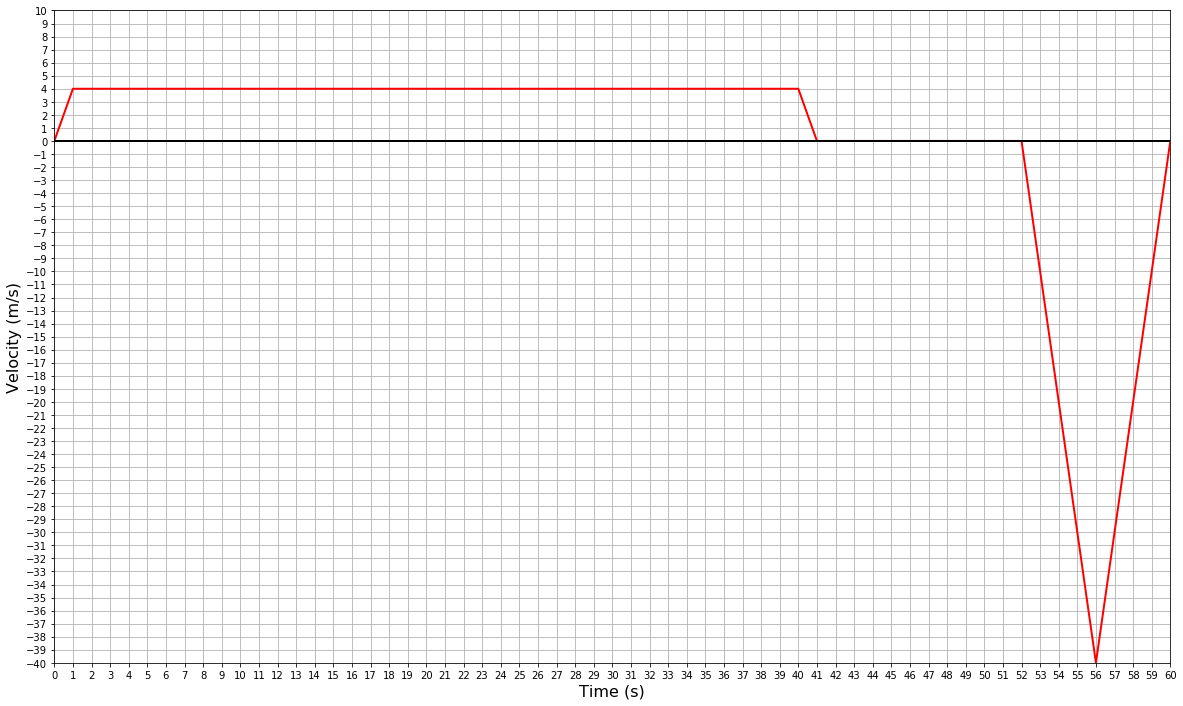
\includegraphics[width=0.7\textwidth]{../images/test1V1_dropTower.png}
\end{center}

\begin{parts}
	\part[2] When is \textit{acceleration zero} during the ride? Provide all time interval(s).
		\begin{TheSolution}
			Acceleration is zero when velocity is unchanging (and so the line is flat in the above graph). This happens (1) between t=1s and t=40s and (2) between t=41s and t=52s.
		\end{TheSolution}
	\part[2] When do people experience free fall during the ride (i.e. are accelerating solely due to gravity)? Provide all time interval(s).
		\begin{TheSolution}
			They are experiencing free fall between t=51s and t=55s (their acceleration is $-10 m/s^2$).
		\end{TheSolution}
	\part[2] How high is the tower?
		\begin{TheSolution}
			The area under a velocity versus time graph provides displacement. To find the height of the tower, we can look at the area under the curve from t=0s to t=41s or between t=52s to t=60s (both will give the same answer).
			\begin{eqnarray}
				Area (rectangle) = base \times height = 40s \times 4m/s = 160m \\
				Area (triangle) = \frac{1}{2} base \times height = \frac{1}{2} 8s\times -40s = -160m
			\end{eqnarray}
		\end{TheSolution}
\end{parts}
\end{minipage}

\clearpage

\bonusquestion[4] List 4 problems with science.
\begin{TheSolution}
	There are a great many possible answers to this question. Some of the ones we covered in the first class include:
\begin{itemize}
	\item People have a tendency to double down on their opinions, rather than change them, when faced with contradicting evidence
\item People have biases and perspectives that prevent objectivity
\item People want the glory of a new discovery, therefore little effort is put into verifying experimental results.
\item ``Science" is seen as pure and objective, and associated with hard reasoning. It is therefore difficult to challenge an ``expert scientist" who can wield their titled when questioned (about motives, intention), conferring a position of authority
\item Science funding often dictates science project.
\end{itemize}
\end{TheSolution}


\end{questions}


\end{document}